\section{Installation \& Setup}
\justifying
\begin{tcolorbox}[colback=green!5!white,colframe=green!75!black,width=\textwidth]
Note: ColumnFlown only runs on Linux and may require up to 4 GB of disc space. \tcblower
Also, the machine where you run this exercise must be mounted with CERN AFS.
\end{tcolorbox}

Start by going to the GitLab repository of this exercise: 

\texttt{\textcolor{LimeGreen}{\href{https://gitlab.cern.ch/cms-analysis/analysisexamples/columnflow-demo}{\underline{https://gitlab.cern.ch/cms-analysis/analysisexamples/columnflow-demo}}}}

To have your own copy of the code, fork the repository into your personal area. You can do this by clicking the \code{Fork} button on the upper right corner of the page. To set your Project URL please type your CERN username in the \code{Select a namespace} option. 

\begin{figure}[!h]
    \centering
    \includegraphics[scale=0.62]{images/gitlab.png}
\end{figure}
\begin{figure}[!h]
    \centering
    \includegraphics[scale=0.62]{images/fork1.png}
\end{figure}

After clicking the \code{Fork project} button, your fork url should be:

\texttt{https://gitlab.cern.ch/<cern\_username>/columnflow-demo}

\newpage
In your forked project, go to the \code{Code} button on the right hand side of the page and copy the address under the \code{Clone with HTTPS} option. If you have an SSH key registered on GitLab prior to this exercise, you can also use the \code{Clone with SSH} option. 

\begin{figure}[!h]
    \centering
    \includegraphics[scale=0.62]{images/fork2.png}
\end{figure}

Next, open a new terminal window and clone your code to your machine by running \underline{one of} the following commands (depending on which cloning method you chose):

\begin{lstlisting}[language=bash]
git clone --recursive https://gitlab.cern.ch/<cern_username>/columnflow-demo.git
\end{lstlisting}
\begin{lstlisting}[language=bash]
git clone --recursive ssh://git@gitlab.cern.ch:7999/<cern_username>/columnflow-demo.git
\end{lstlisting}

The directory you have thus created will be referred to as \code{basedir}. You can now go inside your local repository and install ColumnFlow. The \code{setup.sh} bash script will initialize the software environment with \code{micromamba}. Here, we define \code{dev} as the setup name, but you are free to name it as you wish.

\begin{lstlisting}[language=bash]
cd columnflow-demo
source setup.sh dev
\end{lstlisting}

You will be asked to define a series of variables, the first of which is your CERN username. For all other variables you can keep the default name by just pressing \code{Enter}. Variables specific to this exercise will start with \code{H4L\_}, while ColumnFlow specific variables start with \code{CF\_}. You can find all variables in the \code{.setups/dev.sh} bash file. We invite you to check out this file and familiarize yourself with these variables.

\begin{figure}[!h]
    \centering
    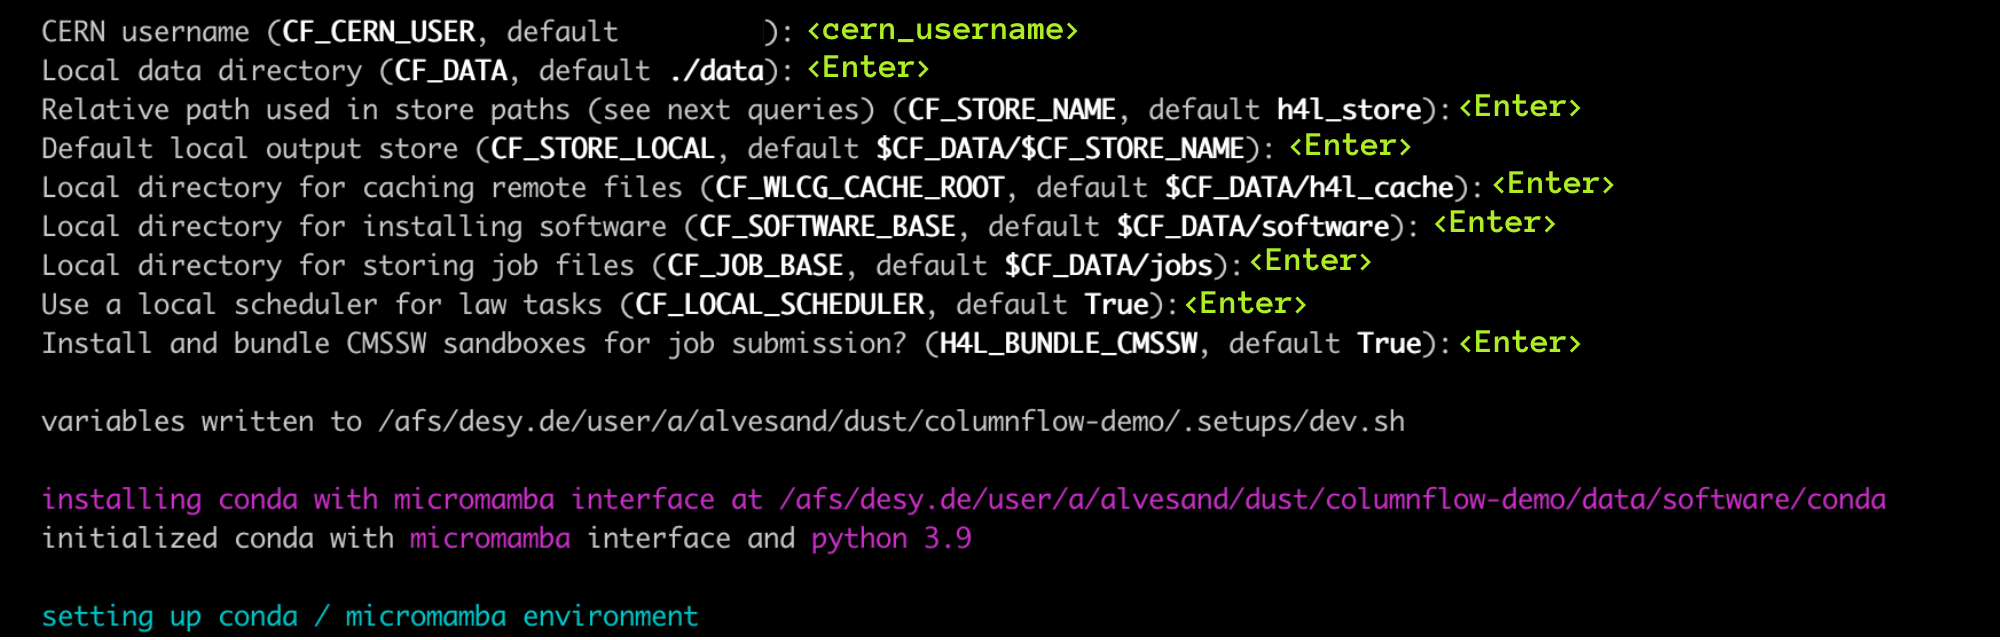
\includegraphics[scale=0.62]{images/setup.png}
\end{figure}

Note that the first installation of the software can take \underline{up to several minutes}. 

Every time you want to work with ColumnFlow (e.g. if you open a new terminal window), you will need to source the \code{setup.sh} script again.

Once the installation is complete you should see a line of green text stating that the analysis has been successfully set up. You are now ready to start working with ColumnFlow! 

\begin{figure}[!h]
    \centering
    \includegraphics[scale=0.62]{images/setup2.png}
\end{figure}

Inside of your newly created \code{columnflow-demo} directory, you will find the following project structure:
\begin{figure}[!h]
    \centering
    \includegraphics[scale=0.62]{images/CF_demo.png}
\end{figure}

\subsection{ColumnFlow Tasks}

This exercise is organized in the form of \code{law} tasks, where different tasks create some form of output. By default, these tasks will save their output on a remote file system (e.g. \texttt{WLGC}), for which you will require a \code{voms-proxy}. If you would like to save certain/all outputs locally, we recommend to create a directory on a system with a larger amount of disk space (e.g. \texttt{EOS}). For such cases, you will need to update the \code{law.cfg} file accordingly. You can view the available tasks by running:
\begin{lstlisting}[language=bash]
law index --verbose
\end{lstlisting}

This exercise will focus on the following tasks:

\begin{itemize}
    \item \texttt{\textcolor{LimeGreen}{cf.CalibrateEvents}} / \texttt{\textcolor{LimeGreen}{cf.SelectEvents}}
    \item \texttt{\textcolor{LimeGreen}{cf.ProduceColumns}}
    \item \texttt{\textcolor{LimeGreen}{cf.PlotCutflow}}
    \item \texttt{\textcolor{LimeGreen}{cf.PlotVariables1D}} / \texttt{\textcolor{LimeGreen}{cf.PlotVariables2D}}
    \item \texttt{\textcolor{LimeGreen}{cf.CreateDatacards}}
\end{itemize}



